%% LyX 2.2.1 created this file.  For more info, see http://www.lyx.org/.
%% Do not edit unless you really know what you are doing.
\documentclass[english,spanish]{extarticle}
\usepackage[T1]{fontenc}
\usepackage{geometry}
\geometry{verbose,tmargin=1in,bmargin=1in,lmargin=1in,rmargin=1.54in}
\setcounter{secnumdepth}{5}
\setcounter{tocdepth}{5}
\setlength{\parskip}{\bigskipamount}
\setlength{\parindent}{0pt}
\usepackage{float}
\usepackage{textcomp}
\usepackage{pdfpages}
\usepackage{amsmath}
\usepackage{graphicx}
\usepackage{setspace}
\usepackage[numbers]{natbib}
\doublespacing

\makeatletter

%%%%%%%%%%%%%%%%%%%%%%%%%%%%%% LyX specific LaTeX commands.
%% A simple dot to overcome graphicx limitations
\newcommand{\lyxdot}{.}


%%%%%%%%%%%%%%%%%%%%%%%%%%%%%% Textclass specific LaTeX commands.
\numberwithin{equation}{section}
\numberwithin{figure}{section}
\numberwithin{table}{section}
 % used for custom paragraph shapes
 \IfFileExists{candleshape.def}{%
  \input{candleshape.def}}{}
 \IfFileExists{dropshape.def}{%
  \input{dropshape.def}}{}
 \IfFileExists{TeXshape.def}{%
  \input{TeXshape.def}}{}
 \IfFileExists{triangleshapes.def}{%
  \input{triangleshapes.def}}{}


\@ifundefined{date}{}{\date{}}
%%%%%%%%%%%%%%%%%%%%%%%%%%%%%% User specified LaTeX commands.
\date{}
%\usepackage{setspace}
%\doublespacing
\usepackage[nottoc,notlof,notlot]{tocbibind} % Put the bibliography in the ToC
\usepackage{listings}
\usepackage{color}

\usepackage{tikz}
\usetikzlibrary{dsp,chains}
\DeclareMathAlphabet{\mathpzc}{OT1}{pzc}{m}{it}
\newcommand{\z}{\mathpzc{z}}
\newcommand{\TikZ}{Ti\textit{k}Z\xspace}

\makeatother

\usepackage{babel}
\addto\shorthandsspanish{\spanishdeactivate{~<>}}

\usepackage{listings}
\begin{document}
\includepdf{pdf/portada}

\newpage{}


\title{Hoja de Aprobaci\'{o}n.}

\maketitle
\thispagestyle{empty} 

\newpage{}



\title{\textbf{Uso de Simulink y la Tarjeta de desarrollo Atlys de Xilinx
para la implementaci\'{o}n de Sistemas de Procesamiento de Se\~{n}ales
e im\'{a}genes.}}

\maketitle
\vspace{1cm}

\begin{center}
Diego Armando Hern\'{a}ndez Ram\'{\i}rez.
\par\end{center}

\begin{center}
\textbf{Asesor t\'{e}cnico:} Mtro. Jos\'{e} Mar\'{\i}a Valencia Velasco.
\par\end{center}

\begin{center}
\textbf{Asesor metodol\'{o}gico:} Mtro. Cuauht\'{e}moc Rafael Aguilera
Galicia.
\par\end{center}

\thispagestyle{empty} 

\newpage{}



\title{Agradecimientos}

\maketitle
\thispagestyle{empty} 

\newpage{}


\begin{spacing}{1}

\tableofcontents{}

\listoftables

\listoffigures

\end{spacing}

\newpage{}

\setlength{\parindent}{12pt}

\begin{doublespace}

\part{Introducci\'{o}n.}
\end{doublespace}
\begin{doublespace}

\section{Planteamiento del problema.}
\end{doublespace}

En la actualidad la electr\'{o}nica est\'{a} presente en pr\'{a}cticamente
en todos los aspectos de nuestra vida a trav\'{e}s de una gran infinidad
de dispositivos y sistemas: tel\'{e}fonos inteligentes, monitores
de ritmo cardiaco, c\'{a}maras fotogr\'{a}ficas, televisores, autom\'{o}viles,
refrigeradores, computadoras, etc. 

Todos estos dispositivos realizan de manera interna la manipulaci\'{o}n
e interpretaci\'{o}n de se\~{n}ales el\'{e}ctricas, que en otras palabras
es lo que se conoce como procesamiento de se\~{n}ales. El procesamiento
de una se\~{n}al puede aplicarse, por ejemplo, en el reconocimiento
de voz para determinar qui\'{e}n es la persona que habla; para determinar,
mediante una imagen, piezas defectuosas en una l\'{\i}nea de producci\'{o}n
o para la protecci\'{o}n de informaci\'{o}n (encriptaci\'{o}n). 

El procesamiento de se\~{n}ales involucra la realizaci\'{o}n de operaciones
matem\'{a}ticas sobre las se\~{n}ales, las cuales son llevadas por
sistemas cuya \'{u}nica funci\'{o}n es precisamente el llevar a cabo
esas operaciones, los procesadores digitales de se\~{n}ales (DSP,
por sus siglas en ingl\'{e}s) y los arreglos programables (FPGA, por
sus siglas en ingl\'{e}s) son los encargados de ello. 

En muchas aplicaciones de procesamiento de se\~{n}ales se requiere
una velocidad de procesamiento elevada (por ejemplo procesamiento
de video) por lo que, debido al paralelismo de su operaci\'{o}n, los
FPGA son aptos para ser utilizados en ellas\cite{kehtarnavaz_digital_2010}. 

Con el fin de explotar las ventajas que los FPGA poseen y poderlos
aplicar de una manera eficaz en el procesamiento de se\~{n}ales es
necesario contar con s\'{o}lidos conocimientos principalmente en metodolog\'{\i}as
de dise\~{n}o digital e implementaci\'{o}n matem\'{a}tica de algoritmos;
estos conocimientos deben adquirirse desde la academia, puesto que
es el tiempo ideal en que el futuro ingeniero o arquitecto de sistemas
puede ir desarrollando, a trav\'{e}s de la experimentaci\'{o}n, las
habilidades necesarias para crear prototipos en el que se involucre
el procesamiento de se\~{n}ales. 

Teniendo como objetivo principal el recortar la curva de aprendizaje,
las empresas l\'{\i}deres en FPGA como Xilinx, Altera y Synopsys proporcionan
plataformas de trabajo que puede interactuar con Matlab (software
especializado que permite la implementaci\'{o}n y prueba de algoritmos).
De esta forma, el alumno puede poner en pr\'{a}ctica de forma \'{a}gil
y sin complicaciones los conocimientos adquiridos en las \'{a}reas
de procesamiento digital de se\~{n}ales. 

Muchas veces la informaci\'{o}n que el fabricante proporciona sobre
sus plataformas de trabajo es escasa y poco concreta, lo que puede
impactar negativamente en el inter\'{e}s del alumno, provocando que
los conocimientos y conceptos no queden del todo entendidos. 

\section{Revisi\'{o}n de la literatura.}

\section{Prop\'{o}sito.}
\begin{doublespace}

\subsection{Objetivo general.}
\end{doublespace}
\begin{itemize}
\begin{doublespace}
\item Describir el proceso de implementaci\'{o}n de un sistema de procesamiento
de se\~{n}ales e im\'{a}genes mediante hardware reconfigurable (FPGA)
y la tarjeta de desarrollo Atlys.
\end{doublespace}
\end{itemize}
\begin{doublespace}

\subsection{Objetivos espec\'{\i}ficos.}
\end{doublespace}
\begin{itemize}
\begin{doublespace}
\item Facilitar el dise\~{n}o e implementaci\'{o}n de un sistema de procesamiento
de audio en tiempo real, basado en el desarrollo de un algoritmo de
eco, as\'{\i} como un sistema de detecci\'{o}n de bordes en una imagen
basado en el algoritmo Sobel, ambos utilizando bloques de Xilinx System
Generator para Simulink.
\item Mostrar la conversi\'{o}n de los algoritmos matem\'{a}ticos b\'{a}sicos
que intervienen en el procesamiento de se\~{n}ales, a hardware en
FPGA, haciendo uso de la abstracci\'{o}n que proporciona Simulink
\item Describir las t\'{e}cnicas de implementaci\'{o}n m\'{a}s eficientes
para obtener el mayor rendimiento sobre la familia FPGA Spartan 6
utilizada en la tarjeta Atlys
\item Dise\~{n}ar las propiedades intelectuales (IPs) m\'{a}s comunes en
el tratamiento de se\~{n}ales tales como bloques de filtros FIR, IIR
y convoluciones, utilizando los entornos de programaci\'{o}n de MATLAB\textregistered{}
y Xilinx\textregistered .
\item Explicar los diferentes m\'{e}todos de ejecuci\'{o}n del hardware
dise\~{n}ado en Simulink\textregistered , sobre la tarjeta Atlys. 
\item Justificar el uso de MATLAB/Simulink\textregistered{} y Xilinx/ISE\textregistered{}
para el dise\~{n}o e implementaci\'{o}n de algoritmos complejos en
contraste con el uso tradicional de HDL puro.
\end{doublespace}
\end{itemize}
\newpage{}



\part{Antecedentes.}

\section{Procesamiento Digital de Se\~{n}ales.}

\subsection{Elementos de un sistema DSP.}

El procesamiento digital de se\~{n}ales es una de las tecnolog\'{\i}as
m\'{a}s vanguardistas que ha marcado varios segmentos tecnol\'{o}gicos
como las comunicaciones digitales, ciencias m\'{e}dicas, dise\~{n}o
de radares, reproductores de m\'{u}sica de alta fidelidad, por nombrar
s\'{o}lo algunas. Esta \'{a}rea se distingue de todas las dem\'{a}s
dentro de las Ciencias de la Computaci\'{o}n, por el tipo de datos
\'{u}nico que utiliza: \textbf{las se\~{n}ales \cite{New1}. }

El prop\'{o}sito principal de un sistema de procesamiento digital
de se\~{n}ales es manipular matem\'{a}ticamente alg\'{u}n tipo de
informaci\'{o}n tomada del mundo real. Dicha informaci\'{o}n es naturalmente
anal\'{o}gica, es decir, la representaci\'{o}n de sus valores y funciones
son continuos, por lo que necesita ser previamente digitalizada antes
de ser procesada. Algunos ejemplos de se\~{n}ales com\'{u}nmente utilizados
son voz, audio, video, temperatura y presi\'{o}n. 

Generalmente las operaciones que se realizan sobre dichas se\~{n}ales
son adiciones, sustracciones, multiplicaciones y divisiones, mismas
que se deben ejecutar muy r\'{a}pidamente con el fin de generar una
salida mucho m\'{a}s precisa\cite{analog_devices}. Esto se hace para
cumplir una amplia variedad de objetivos, tales como: mejoras en la
visualizaci\'{o}n de im\'{a}genes, reconocimiento y generaci\'{o}n
de voz, compresi\'{o}n de datos para almacenamiento y transmisi\'{o}n,
etc. 

El procesamiento digital de se\~{n}ales anal\'{o}gicas puede ser descrito
en tres etapas:
\begin{itemize}
\begin{doublespace}
\item La se\~{n}al anal\'{o}gica es \emph{digitalizada}, es decir, se \emph{muestrea}
y cada muestra es a su vez, \emph{cuantizada} a un n\'{u}mero finito
de bits. Este proceso es llamado \textbf{conversi\'{o}n anal\'{o}gico-digital}.
\item Los muestreos digitalizados son procesados por un \emph{Procesador
Digital de Se\~{n}ales}.
\item Las muestras resultantes de la etapa de procesamiento, se convierten
de nuevo a un formato \emph{anal\'{o}gico} mediante alguna t\'{e}cnica
de reconstrucci\'{o}n anal\'{o}gica (\textbf{conversi\'{o}n digital-anal\'{o}gico}).
\end{doublespace}
\end{itemize}

\begin{doublespace}
Un sistema DSP t\'{\i}pico se muestra en la Figura \ref{fig:Diagrama-a-bloques}.
\end{doublespace}

\begin{figure}[H]
\begin{centering}
\includegraphics[scale=0.4]{img/fullblocks}
\par\end{centering}
\caption{Diagrama a bloques de un Sistema de procesamiento Digital de Se\~{n}ales.\label{fig:Diagrama-a-bloques}}

\end{figure}

Las secciones a continuaci\'{o}n describen con m\'{a}s detalle, los
teoremas y t\'{e}cnicas fundamentales que intervienen en los sistemas
DSP.

\subsubsection{Teorema de muestreo.}

El \emph{teorema de muestreo} establece que para una representaci\'{o}n
precisa de una se\~{n}al $\mathbf{x(t)}$ por sus muestras de tiempo
$\mathbf{x(nT)}$, dos condiciones deben cumplirse:
\begin{itemize}
\item La se\~{n}al $\mathbf{x(t)}$ debe ser de banda limitada, es decir,
su espectro de frecuencia debe ser limitada para contener las frecuencias
hasta cierta frecuencia m\'{a}xima, digamos $\mathbf{f_{max}}$, y
sin frecuencias m\'{a}s all\'{a} de eso. Un espectro t\'{\i}pico de
banda limitada se muestra en la Figura \ref{fig:Banda-de-espectro}.
\item La frecuencia de muestreo $\mathbf{f_{s}}$debe ser elegida para ser
al menos el doble de la frecuencia m\'{a}xima $\mathbf{f_{s}}$, es
decir,
\begin{equation}
\mathbf{f_{s}\leq2f_{max}}
\end{equation}
\item En t\'{e}rminos del intervalo del tiempo de muestreo:
\begin{equation}
\mathbf{T\leq\frac{1}{2f_{max}}}
\end{equation}
\end{itemize}
\begin{figure}[H]
\begin{centering}
\includegraphics[scale=0.7]{img/sampling_theorem}
\par\end{centering}
\caption{Banda de espectro limitado t\'{\i}pica \cite{dsp_introduction}.\label{fig:Banda-de-espectro}}

\end{figure}

La velocidad de muestreo m\'{\i}nima permitida por el teorema de muestreo,
que es $\mathbf{f_{s}=2f_{max}}$, es llamada \emph{Tasa de muestreo
de Nyquist. }Para valores arbitrarios de $\mathbf{f_{s}}$, la magnitud
de $\mathbf{\mathbf{\frac{f_{s}}{2}}}$ es llamada \emph{Frecuencia
de Nyquist}\textbf{\emph{. }}Esta frecuencia tambi\'{e}n define\textbf{
}las frecuencias de corte de los filtros pasa bajas que se requieren
en las operaciones en DSP-.

\subsubsection{Cuantizaci\'{o}n.}

El muestreo y la cuantizaci\'{o}n son requisitos indispensables para
cualquier operaci\'{o}n de procesamiento digital en se\~{n}ales anal\'{o}gicas.
Una se\~{n}al digital es una secuencia de n\'{u}meros\footnote{Esta secuencia es conocida como \textbf{Muestra.}}
en donde cada muestra es representada por un n\'{u}mero finito de
digitos\footnote{En el dise\~{n}o de sistemas DSP, se dice que la se\~{n}al es de \textbf{precisi\'{o}n
finita} cuando la representaci\'{o}n est\'{a} dada por un n\'{u}mero
finito de datos.}.La cuantizaci\'{o}n es el proceso de convertir una se\~{n}al discreta
en el tiempo de amplitud continua, a una se\~{n}al digital, representando
cada valor muestreado como un n\'{u}mero finito de digitos. La Figura
\ref{fig:Ejemplo-de-cuantizaci=0000F3n} muestra la representaci\'{o}n
gr\'{a}fica de una se\~{n}al cuantizada.

\begin{figure}[H]
\begin{centering}
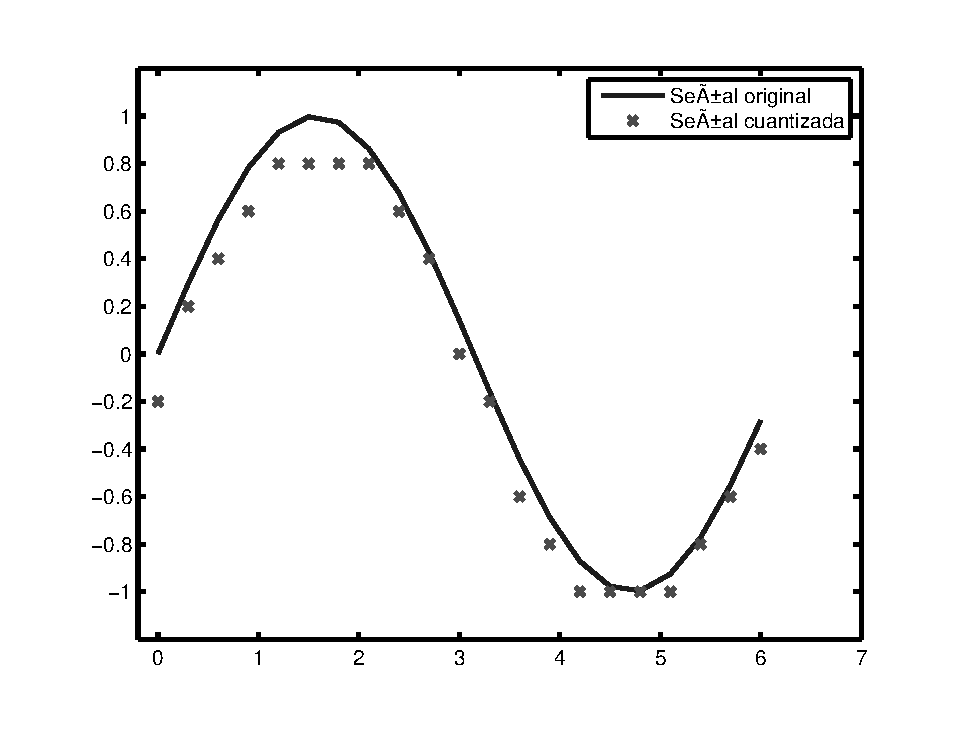
\includegraphics[scale=0.5]{img/quantization_example}
\par\end{centering}
\caption{Ejemplo de cuantizaci\'{o}n en una se\~{n}al senoidal. Los puntos
marcados con una <<x>> representan la se\~{n}al original, mientras
que las coordenadas marcadas con <<\textendash >> muestran la se\~{n}al
cuantizada \label{fig:Ejemplo-de-cuantizaci=0000F3n}.}

\end{figure}

Este proceso induce un error llamado \emph{error de} \emph{cuantizaci\'{o}n,
}el cual se debe al cambio en la representaci\'{o}n de la se\~{n}al
original, de un valor continuo a un set de valores discretos. En t\'{e}rminos
matem\'{a}ticos, la operaci\'{o}n de cuantizaci\'{o}n de las muestras
$\mathit{\mathbf{x(n)}}$ se denota como $\mathbf{Q[x(n)]}$. Tomando
$\mathbf{x_{q}(n)}$ como la secuencia de muestras cuantizadas, el
sistema completo queda como:

\begin{equation}
\mathbf{x_{q}(n)}\mathbf{=Q[x(n)]}
\end{equation}

El error de cuantizaci\'{o}n es representado por la secuencia $\mathbf{e_{q}(n)}$,
como la diferencia entre los valores cuantizados y el valor de la
muestra actual:

\begin{equation}
\mathbf{e_{q}x(n)=x_{q}(n)-x(n)}
\end{equation}


\subsection{Sistemas Discretos Lineales e Invariantes en el Tiempo..}

La relaci\'{o}n entrada/salida de de los sistemas \emph{Lineales e
Invariantes en el Tiempo} (LTI, por sus siglas en ingl\'{e}s) est\'{a}
definida por la \emph{convoluci\'{o}n }en tiempo discreto de la respuesta
del impulso finito aplicado a la entrada del sistema.

Los sistemas LTI pueden ser clasificados en dos tipos, dependiendo
de si su respuesta al impulso tiene duraci\'{o}n finita o infinita,
estos son:\emph{ Respuesta al Impulso Finito} (FIR, por sus siglas
en ingl\'{e}s) o \emph{Respuesta al Impulso Infinito} (IIR, por sus
siglas en ingl\'{e}s).

En t\'{e}rminos matem\'{a}ticos, se dice que un sistema es lineal
cuando, por ejemplo, dos se\~{n}ales de entrada $\mathbf{x_{1}(t)}$
y $\mathbf{x_{2}(t)}$ tienen salidas $\mathbf{y_{1}(t)}$ y $\mathbf{y_{2}(t)}$
respectivamente. Entonces, la salida del sistema al impulso $\mathbf{\alpha_{1}x_{1}(t)+\alpha_{2}x_{2}(t)}$
es $\mathbf{\alpha_{1}y_{1}(t)+\alpha_{2}y_{2}(t)}$. Es decir, cumplen
con las reglas de \emph{homogeneidad }y \emph{superposici\'{o}n.}

Tambi\'{e}n, un sistema es invariante en el tiempo cuando $\mathbf{y(t)}$
es la salida correspondiente a $\mathbf{x(t)}$, entonces para cada
\textbf{\ensuremath{\tau}}, $\mathrm{\mathbf{y(t-\tau)}}$ es la salida
que corresponde a $\mathbf{x(t-\tau)}$. Es decir, si agregamos un
retraso a la entrada o salida, el resultado debe ser exactamente el
mismo.

Adem\'{a}s, los \emph{sistemas LTI}\textbf{\emph{ }}deben ser causales,
lo que significa que la salida del sistema no puede anticipar la entrada
del mismo, tal que, para todo impulso de entrada $\mathbf{\delta(t)}$,
la salida $\mathbf{h(t)=0}$ mientras $\mathbf{t<0}$ .

Otra caracter\'{\i}stica que debe cumplir, es la de ser un sistema
sin memoria. Se dice que un sistema tiene memoria cuando la se\~{n}al
de salida depende de las entradas pasadas y/o futuras. Por ejemplo,
la ecuaci\'{o}n del c\'{a}lculo del voltaje de un resistor representa
un sistema sin memoria dado que $\mathbf{v(t)=Ri(t)}$, mientras que
el voltaje en un capacitor representa un sistema con memoria por su
ecuaci\'{o}n $\mathbf{v(t)=v(t_{0})+\int_{t_{0}}^{t}i(\tau)d\tau}$.

En t\'{e}rminos de hardware, todos los \emph{sistemas LTI} pueden
ser implementados a base de sumadores, multiplicadores y unidades
de retraso. Estos sistemas son facilmente realizables dado que se
basan a partir de un n\'{u}mero finito de elementos, como los antes
mencionados.

Las siguientes subsecciones resumen conceptos importantes que son
utilizados en cualquier aplicaci\'{o}n y dise\~{n}o de sistemas DSP.

\subsubsection{Convoluci\'{o}n.}

La convoluci\'{o}n es la forma matem\'{a}tica de combinar dos se\~{n}ales
para formar una tercera. Es la t\'{e}cnica m\'{a}s importante en el
Procesamiento Digital de Se\~{n}ales. Usando la estrategia de la descomposici\'{o}n
del impulso, los sistemas pueden ser descritos por una se\~{n}al llamada
\emph{respuesta al impulso.} La convoluci\'{o}n es importante porque
relaciona las tres se\~{n}ales de inter\'{e}s: la se\~{n}al de entrada,
la se\~{n}al de salida y la se\~{n}al de respuesta al impulso. 

Un punto fundamental a comprender de los sistemas DSP, es que estos
trabajan descompiniendo la se\~{n}al de entrada en simples componentes
aditivos, cada uno de estos componentes se pasa a trav\'{e}s de un
sistema linear, y los componentes de salida resultantes son sintetizados,
o en otras palabras, sumados. Esta descomposici\'{o}n se puede hacer
de dos formas distintas: \emph{Descomposici\'{o}n por impulsos}\textbf{\emph{
}}y \emph{Descomposici\'{o}n por el m\'{e}todo de Fourier. }Cuando
la Descomposici\'{o}n por impulsos es utilizada, el procedimiento
se puede describir matem\'{a}ticamente utilizando la \textbf{convoluci\'{o}n.}

Esta operaci\'{o}n se basa en dos t\'{e}rminos importantes en los
sistemas DSP. El primero es la \textbf{funci\'{o}n delta, }simbolizada
por $\mathbf{\mathbf{\mathbf{\delta}[n]}}$ . La funci\'{o}n delta
es un impulso normalizado, que es, la muestra n\'{u}mero cero con
un valor asignado de una unidad, mientras que las otras muestras tienen
asignadas un valor de cero. Por esta raz\'{o}n, la funci\'{o}n delta
es llamada \textbf{unidad de impulso.} 

\begin{figure}[H]
\begin{centering}
\includegraphics[scale=0.9]{img/delta}
\par\end{centering}
\caption{Funci\'{o}n \foreignlanguage{english}{delta graficada.}}

\end{figure}

Por otra parte, la \textbf{respuesta al impulso} es la se\~{n}al que
existe en el sistema cuando una funci\'{o}n delta es aplicada a la
entrada. Si dos sistemas son diferentes en cualquier manera, ambos
tendr\'{a}n diferentes respuestas al impulso. Comunmente, las respuestas
a la entrada y salida son llamadas $\mathbf{x[n]}$ y $\mathbf{y[n]}$,
la respuesta al impulso es usualmente llamada $\mathbf{h[n]}$. 

\begin{figure}[H]
\begin{centering}
\includegraphics[scale=0.9]{img/impulse}
\par\end{centering}
\caption{Funci\'{o}n \foreignlanguage{english}{de respuesta al impulso graficada.}}
\end{figure}

En otras palabras, una se\~{n}al de entrada $\mathbf{x[n]}$ , entra
en un sistema linear con una respuesta al impulso $\mathbf{h[n]}$,
resultando en una se\~{n}al de salida $\mathbf{y[n]}$ . En forma
matem\'{a}tica, la ecuaci\'{o}n de convoluci\'{o}n de una sola muestra
queda como se muestra a continuaci\'{o}n:

\begin{equation}
\mathbf{y[n]=x[n]*y[n]}
\end{equation}

Tomando la ecuaci\'{o}n 4.5 como gu\'{\i}a, siendo $\mathbf{x[n]}$
una se\~{n}al de \emph{N} puntos, desplaz\'{a}ndose desde 0 a \emph{N-1},
y $\mathbf{h[n]}$ una se\~{n}al de \emph{M} puntos desplaz\'{a}ndose
de 0 a \emph{M-1}\cite{dspguide_conv} , la convoluci\'{o}n de ambas
se\~{n}ales es una se\~{n}al \emph{N+M-1}ejecut\'{a}ndose desde 0
a \emph{N+M-2}, esto es:

\begin{equation}
\mathbf{y[i]=\sum_{j=0}^{M-1}h[j]}\mathbf{x[i-j]}
\end{equation}

La ecuaci\'{o}n anterior representa la definici\'{o}n formal de la
convoluci\'{o}n, la cual tambi\'{e}n es conocida como la \emph{suma
de convoluci\'{o}n} o \emph{convoluci\'{o}n discreta.}

Un ejemplo de la convoluci\'{o}n tomando como vectores de entrada
$\mathbf{\overrightarrow{v}_{actual}=[v_{1,}v_{2}...}\mathbf{v_{n}]}$
y $\mathbf{\overrightarrow{v}_{anterior}=[v_{n,}v_{n-1}...}\mathbf{v_{1}]}$
se muestra en la \textbf{Figura \ref{fig:Convoluci=0000F3n-de-dos}. }

En el \textbf{Ap\'{e}ndice D} se muestra el script interactivo que
se puede ejecutar en el ambiente de Matlab, el cual fue tomado de
\cite{eece_matlab} . Este script muestra el resultado de la convoluci\'{o}n
discreta de dos impulsos $\mathbf{y[n]=\delta[n]*\delta[n-1]}$ ,
tomando como vector a $\mathbf{n=[1,0,1]}$.

\begin{figure}[H]
\begin{centering}
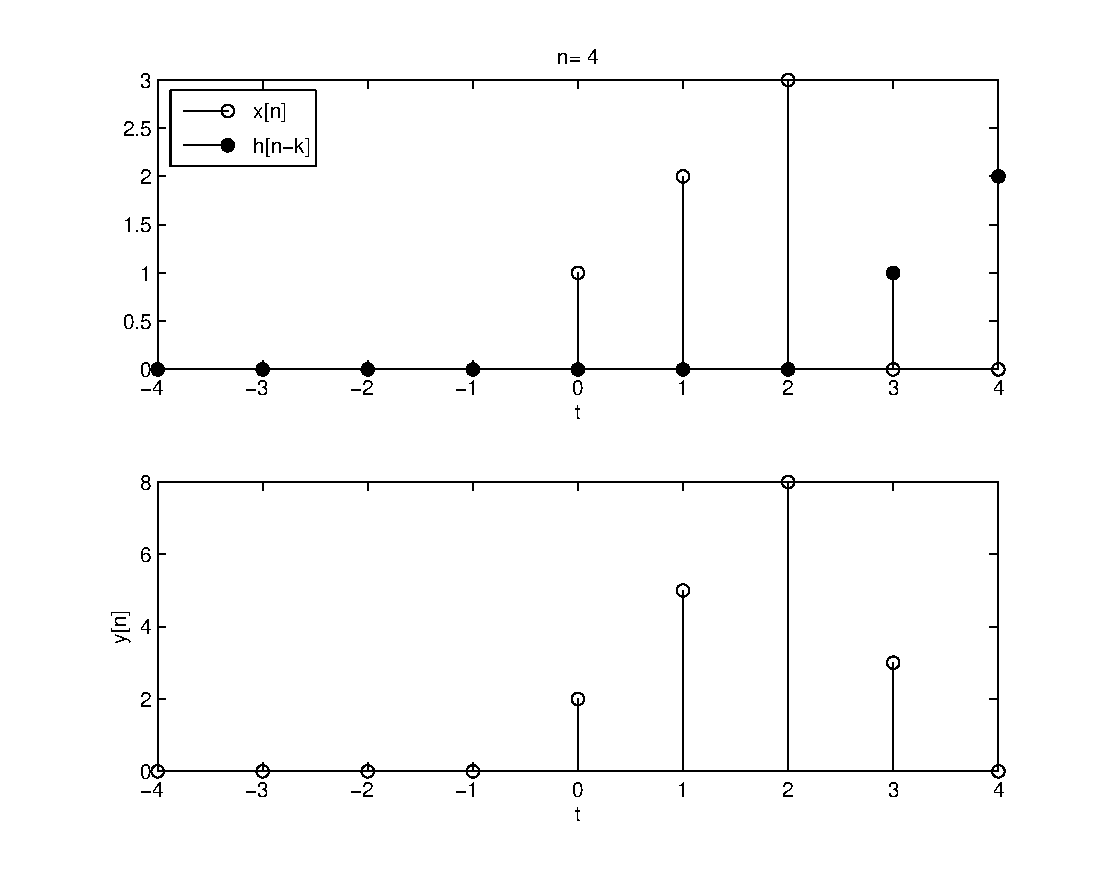
\includegraphics[scale=0.6]{img/convolve}
\par\end{centering}
\caption{\label{fig:Convoluci=0000F3n-de-dos}Convoluci\'{o}n de dos vectores
en Matlab.}

\end{figure}


\subsubsection{Filtros FIR.}

Un filtro digital de \emph{Respuesta Finita al Impulso} (FIR) es un
\emph{sistema LTI} si es definido por un conjunto de coeficientes
constantes. La salida de un filtro FIR de \'{o}rden (o longitud) \textbf{L},
a la respuesta de impulso unitario aplicado a la entrada $\mathbf{x[n]}$,
est\'{a} dada por una versi\'{o}n finita de la ecuaci\'{o}n de convoluci\'{o}n,
como se muestra a continuaci\'{o}n:

\begin{equation}
\mathbf{y[n]=f[n]*x[n]=\sum_{k=0}^{L-1}f[k]x[n-k]}
\end{equation}

Para un tren de impulsos en el dominio del tiempo a la entrada $\mathbf{x[n]}$
, la ecuaci\'{o}n queda como:

\begin{equation}
\mathbf{y[n]=b_{0}x(n)+b_{1}x(n-1)+...+b_{M-1}x(n-M+1)}
\end{equation}

\begin{equation}
=\mathbf{\sum_{k=0}^{M-1}b_{k}x(n-k)}
\end{equation}

En otras palabras, la respuesta al impulso consiste s\'{o}lo de respuesta
en los coeficientes, procedida y antecedida por ceros (el filtro producir\'{a}
una respuesta que ir\'{a} decayendo a cero y se mantendr\'{a} en ese
estado, de ah\'{\i} el nombre caracter\'{\i}stico de este filtro).
Matem\'{a}ticamente se puede expresar esta respuesta al impulso con
la siguiente ecuaci\'{o}n:

\begin{equation}
\mathbf{h(n)=\begin{cases}
b_{n}, & 0\leq n\leq M-1\\
0, & otros
\end{cases}}
\end{equation}

Gr\'{a}ficamente, esta ecuaci\'{o}n se puede representar como se muestra
en la \textbf{Figura \ref{fig:Respuesta-al-impulso}.}

\begin{figure}[H]
\begin{centering}
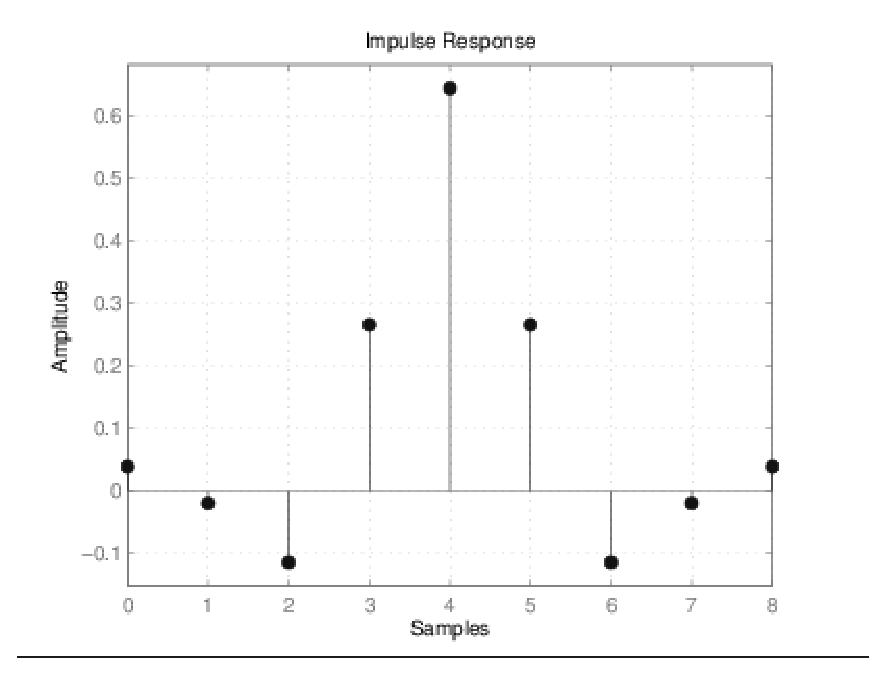
\includegraphics[scale=0.6]{img/fir_filter_impulseresponse_gray}\caption{Respuesta al impulso de un filtro FIR con $\mathbf{b_{0}=0.9}$. \label{fig:Respuesta-al-impulso}}
\par\end{centering}
\end{figure}

Este tipo de filtros son m\'{a}s populares en cuanto a implementaci\'{o}n,
dado que cuentan con caracter\'{\i}sticas muy \'{u}tiles, entre las
cuales destacan:
\begin{itemize}
\item \textbf{\emph{Fase Lineal: }}Esta propiedad implica que la fase es
una funci\'{o}n lineal de la frecuencia, Esto asegura que las se\~{n}ales
de todas las frecuencias se retrasan en la misma cantidad de tiempo,
eliminando la posibilidad de distorsi\'{o}n de fase.
\item \textbf{\emph{Estabilidad:}} Para una entrada finita, la salida siempre
es finita, adem\'{a}s son no recursivos, es decir, no hay una conexi\'{o}n
de retroalimentaci\'{o}n envuelta en la estructura del filtro.
\end{itemize}
Existen muchos m\'{e}todos de implementaci\'{o}n de esto filtros,
la estructura m\'{a}s b\'{a}sica es conocida como \emph{forma directa,
}la cual consta de utilizar la ecuaci\'{o}n en diferencia, no recursiva,
mostrada en (4.7)\cite{fir_complete}, lo que es equivalente a la
sumatoria convolucional. La estructura se muestra en la \textbf{Figura
\ref{fig:Estructura-en-Forma}}, el cual representa un filtro con
un n\'{u}mero de coeficientes $\mathbf{b_{0..3}+1}$\textbf{.}

\begin{figure}[H]
\begin{centering}
% FIR filter as block diagram
\begin{tikzpicture}

	% Place nodes using a matrix
	\matrix[row sep=2.5mm, column sep=5mm]
	{
		%--------------------------------------------------------------------
		\node[dspnodeopen,dsp/label=above] (m00) {$x[n]$};    &
		\node[coordinate]                  (m01) {};          &
		\node[dspnodefull]                 (m02) {};          &
		\node[dspsquare]                   (m03) {$\z^{-1}$}; &
		\node[dspnodefull]                 (m04) {};          &
		\node[dspsquare]                   (m05) {$\z^{-1}$}; &
		\node[dspnodefull]                 (m06) {};          &
		\node[dspsquare]                   (m07) {$\z^{-1}$}; &
		\node[coordinate]                  (m08) {};          &
		\node[coordinate]                  (m09) {};          &
		\node[coordinate]                  (m0X) {};          \\
		%--------------------------------------------------------------------
		\node[coordinate]                  (m10) {};          &
		\node[coordinate]                  (m11) {};          &
		\node[dspmixer, dsp/label=right]   (m12) {$b[0]$};    &
		\node[coordinate]                  (m13) {};          &
		\node[dspmixer, dsp/label=right]   (m14) {$b[1]$};    &
		\node[coordinate]                  (m15) {};          &
		\node[dspmixer, dsp/label=right]   (m16) {$b[2]$};    &
		\node[coordinate]                  (m17) {};          &
		\node[dspmixer, dsp/label=right]   (m18) {$b[3]$};    &
		\node[coordinate]                  (m19) {};          &
		\node[coordinate]                  (m1X) {};          \\
		%--------------------------------------------------------------------
		\\
		%--------------------------------------------------------------------
		\node[coordinate]                  (m20) {};          &
		\node[coordinate]                  (m21) {};          &
		\node[coordinate]                  (m22) {};          &
		\node[coordinate]                  (m23) {};          &
		\node[dspadder]                    (m24) {};          &
		\node[coordinate]                  (m25) {};          &
		\node[dspadder]                    (m26) {};          &
		\node[coordinate]                  (m27) {};          &
		\node[dspadder]                    (m28) {};          &
		\node[coordinate]                  (m29) {};          &
		\node[dspnodeopen,dsp/label=above] (m2X) {$y[n]$};    \\
		%--------------------------------------------------------------------
	};

	% Draw connections
	
	\begin{scope}[start chain]
		\chainin (m00);
		\chainin (m02) [join=by dspflow];
		\chainin (m12) [join=by dspconn];
		\chainin (m22) [join=by dspline];
	\end{scope}

	\foreach \i [evaluate = \i as \j using int(\i+1),
	             evaluate = \i as \k using int(\i+2),] in {2,4,6}
	{
		\begin{scope}[start chain]
			\chainin (m0\i);
			\chainin (m0\j) [join=by dspconn];
			\chainin (m0\k) [join=by dspline];
			\chainin (m1\k) [join=by dspconn];
			\chainin (m2\k) [join=by dspconn];
		\end{scope}
		\draw[dspconn] (m2\i) -- (m2\k);
	}

	\draw[dspflow] (m28) -- (m2X);

\end{tikzpicture}

%\vspace{2em}



\par\end{centering}
\caption{Estructura en Forma Directa de un Filtro FIR\label{fig:Estructura-en-Forma}.
Imagen creada usando el paquete \textup{Ti\textit{k}Z} de \LaTeX }
\end{figure}

En t\'{e}rminos generales, existen cuatro formas b\'{a}sicas de implementaci\'{o}n
de este tipo de filtros, las cuales son:
\begin{itemize}
\item M\'{e}todo por ventanas (Rectangular, Barlett, Hanning, Hamming, Blackman
y Kaiser).
\item Muestreo en frecuencia.
\item Aproximaci\'{o}n de Chebyshev y algoritmo de intercambio de Remez
(conocido como m\'{e}todo de Rizado Constante).
\item M\'{\i}nimos Cuadrados.
\end{itemize}
La implementaci\'{o}n m\'{a}s popular utilizada en FPGA es la del
M\'{e}todo por Ventanas debido a que muchos de los paquetes de software
incluidos en las herramientas de dise\~{n}o de filtros, utilizan este
m\'{e}todo como el principal, lo cual recorta el tiempo de desarrollo
del mismo. 

\subsubsection{Filtros IIR.}

El sistema de Respuesta Infinita al Impulso (\emph{IIR} por sus siglas
en ingl\'{e}s) se caracteriza por utilizar las muestras de la se\~{n}al
de salida en instantes anteriores en adici\'{o}n a las muestras presentes
m\'{a}s las muestras pasadas de la misma funci\'{o}n de salida, es
decir, este filtro cuenta con lazos de \emph{retroalimentaci\'{o}n
}y \emph{anticipaci\'{o}n, }por lo que es conocido como un \textbf{sistema
discreto recursivo}, a diferencia del filtro FIR que se caracteriza
por ser \textbf{no recursivo}.

\subsection{Aplicaciones.}

\section{Tecnolog\'{\i}a FPGA.}

\subsection{Descripci\'{o}n general.}

La Matriz de Compuertas Programables en Campo (FPGA) es un circuito
integrado reconfigurable que puede ser utilizado para dise\~{n}ar
circuitos digitales. La configuraci\'{o}n de la FPGA es normalmente
especificada usando lenguajes de descripci\'{o}n de hardware como
SystemVerilog o VHDL y despu\'{e}s es traducida, mediante herramientas
de s\'{\i}ntesis, a un formato binario en el cual se encuentra la
informaci\'{o}n de ruteo e interconexiones necesarias para que el
dispositivo ejecute las funciones l\'{o}gicas para el cual fue dise\~{n}ado.
Esta propiedad de ser reconfigurable y poder ejecutar m\'{u}ltiples
tareas tan complejas o sencillas, de forma paralela, ofrece una significante
ventaja en muchas aplicaciones como por ejemplo en el dise\~{n}o de
circuitos integrados donde a diferencia del prototipado con ASIC,
en donde los dise\~{n}adores no tienen la flexibilidad de hacer modificaciones
al prototipo despu\'{e}s de que el chip ha sido manufacturado, en
el FPGA es posible y muy com\'{u}n el modificar algunas partes del
circuito despu\'{e}s de que el proyecto ha sido concluido.

La arquitectura de una FPGA se basa en Bloques de Matrices Configurables
(CLBs, por sus siglas en Ingl\'{e}s), las cuales proporcionan la l\'{o}gica
programable y una jerarqu\'{\i}a de interconexiones reconfigurables
para interconectar los CLBs entre s\'{\i}. Adem\'{a}s de estos componentes
b\'{a}sicos, las FPGA actuales contienen bloques de memoria internos,
controladores para interfaces externas de alta velocidad como memorias
DDR y bloques f\'{\i}sicos de PCI Express, as\'{\i} como bloques optimizados
para operaciones de DSP, microprocesadores f\'{\i}sicos y algunas
funciones especiales m\'{a}s, que dependen del enfoque o familia de
la FPGA, todo esto en el mismo silicio.

La tendencia reciente en la tecnolog\'{\i}a FPGA es trabajar con arquitecturas
de hardware en alto nivel de abstracci\'{o}n, agregarle bloques DSP,
procesadores embebidos y transductores de alta velocidad para formar
un Sistema Programable en Chip completo (SoPC). Adem\'{a}s, las FPGA
toman ventaja del paralelismo natural del hardware, ya que exceden
el poder computacional de los Procesadores Digitales de Se\~{n}ales,
rompiendo el paradigma de la ejecuci\'{o}n secuencial y lograr un
mayor rendimiento.

Una de las aplicaciones principales de las FPGA es poder ejecutar
y modificar arquitecturas digitales m\'{u}ltiples veces, hasta que
se ha cumplido el objetivo del prototipo que se estableci\'{o} al
principio, sin ser necesario recurrir a los costosos procesos de fabricaci\'{o}n
de Circuitos Integrados personalizados. Gracias a esto, se pueden
implementar dise\~{n}os de manera incremental e incluso hacer cambios
iterativamente en cuesti\'{o}n de horas en lugar de semanas. Tambi\'{e}n,
debido a la creciente oferta de herramientas de dise\~{n}o en alto
nivel, se ha decrementado la curva de aprendizaje y con frecuencia,
estas herramientas incluyen valiosas Propiedades Intelectuales (IP)
para control y procesamiento de se\~{n}ales avanzadas.

Existe una numerosa cantidad de fabricantes pero s\'{o}lo dos tipos
de FPGAs: Reprogramables (basadas en SRAM o Flash) y Programables
una sola vez (OTP). Las FPGAs basadas en SRAM necesitan una memoria
de configuraci\'{o}n y no retienen los datos cuando son desconectadas
de la fuente de alimentaci\'{o}n. Las que son basadas en Flash, no
necesitan una memoria externa para almacenar la configuraci\'{o}n
y la pueden mantener a\'{u}n cuando el dispositivo no est\'{a} energizado.
Anteriormente, las FPGAs basadas en Flash ten\'{\i}an la caracter\'{\i}stica
de ser OTP, pero hoy en d\'{\i}a existen dispositivos basados en esta
tecnolog\'{\i}a que pueden ser reprogramados tales como las MAX 10
de Altera.

En la pr\'{o}xima secci\'{o}n se cubrir\'{a} a detalle, la arquitectura
de la familia Spartan6 de Xilinx, ya que es esta la que se encuentra
en el kit de desarrollo Atlys de Digilent.

\subsection{Estructura general de las FPGA.}

Como se mencion\'{o} anteriormente, las FPGA modernas ofrecen una
serie de componentes que son de gran utilidad al momento de dise\~{n}ar
sistemas digitales. Estos b\'{a}sicamente son:
\begin{itemize}
\begin{doublespace}
\item Bloques L\'{o}gicos Configurables (CLB) para poder implementar funciones
l\'{o}gicas as\'{\i} como registros.
\item Memoria en Chip (On-chip memory) que provee almacenamiento de datos
dentro del FPGA, generalmente es reducido dado que el \'{a}rea de
construcci\'{o}n de memoria en el silicio, tiende a ocupar gran parte
de este.
\item Propiedades Intelectuales f\'{\i}sicas, tales como controladores Ethernet
MAC, Transductores, Multiplicadores optimizados, bloques DSP, Procesadores,
Controladores de memoria externa DDR, PCIe endpoint f\'{\i}sico, etc.
\item Recursos de manejo de reloj que generen las frecuencias necesarias
para controlar dispositivos como los antes mencionados y que adem\'{a}s,
puedan ser distribuidos dentro de la FPGA. Esto es muy importante
al momento de dise\~{n}ar sistemas con un alto \'{\i}ndice de transferencia
de datos.
\item Bloques de entrada y salida que comuniquen a la FPGA al mundo exterior.
\item Recursos de ruteo para proveer la interconectividad de los Bloques
L\'{o}gicos Configurables internos y las Propiedades Intelectuales.
\end{doublespace}
\end{itemize}
La \textbf{Figura \ref{fig:Arquitectura-general-de}} muestra la arquitectura
t\'{\i}pica de una FPGA con los bloques de construcci\'{o}n b\'{a}sicos.
Es importante mencionar que algunos elementos como las Block RAM,
bloques DSP, controladores de memoria, etc\'{e}tera, que se muestran
en la imagen, son construidos sobre el mismo silicio, sin quitarle
espacio a los elementos l\'{o}gicos. Tambi\'{e}n cabe mencionar que,
las Tablas de B\'{u}squeda, mejor conocidas como Look Up Tables (LUT)
que hay dentro de los bloques l\'{o}gicos son usadas para crear funciones
de l\'{o}gica combinacional, pero tambi\'{e}n pueden ser configuradas
como memorias RAM o registros de desplazamiento. Esta es una forma
muy eficiente de inferir dichos registros sin tener que usar los elementos
de almacenamiento.

\begin{figure}[H]
\begin{centering}
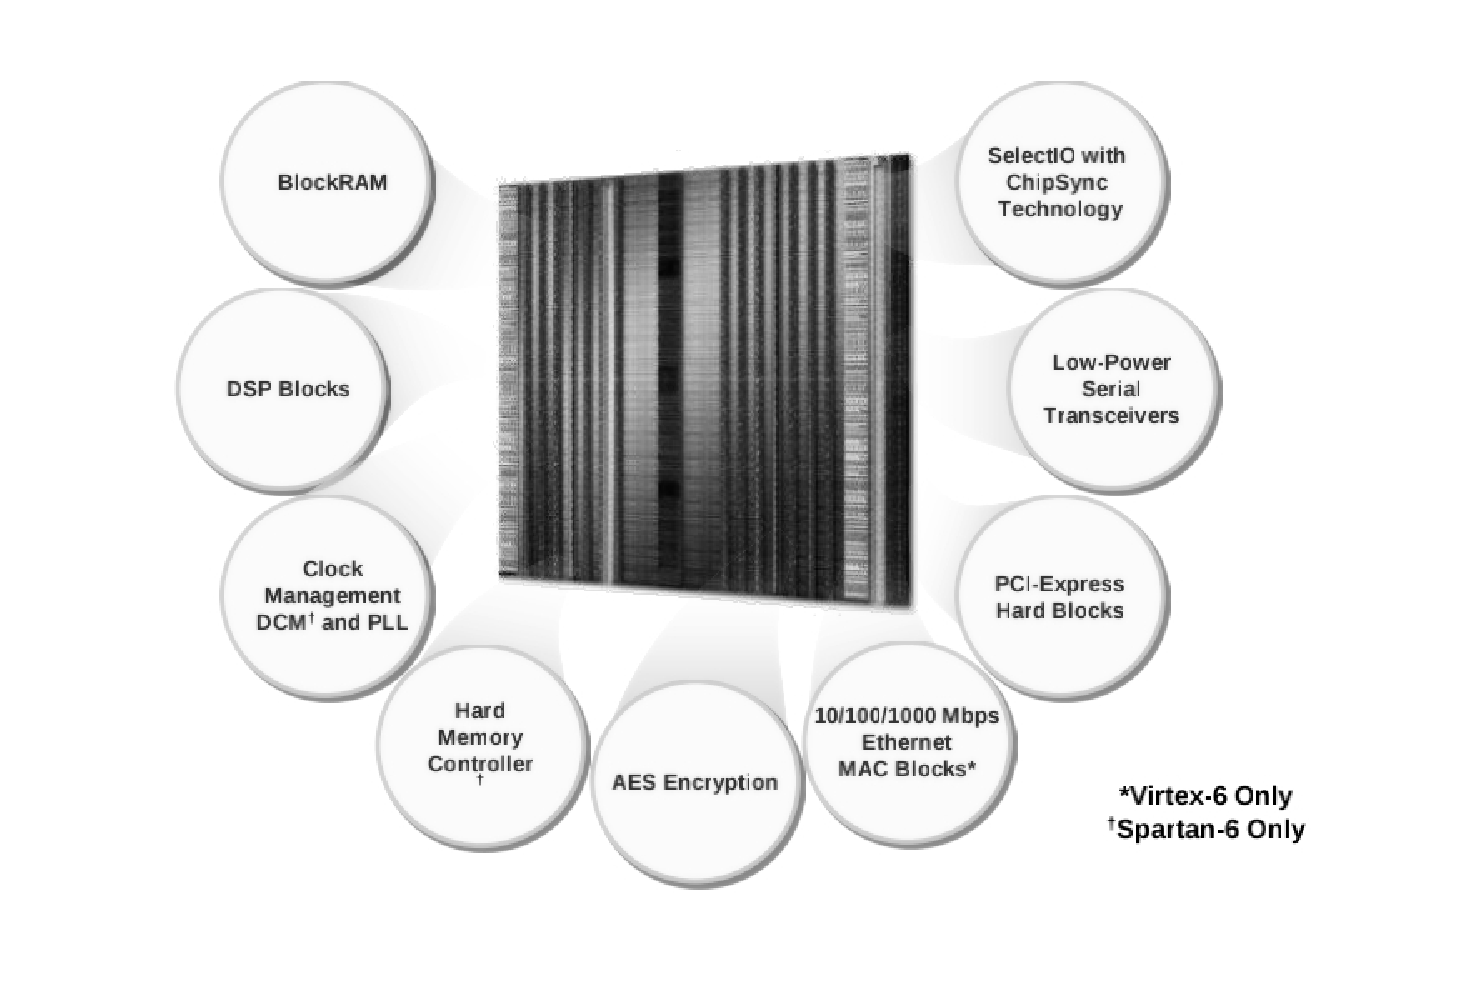
\includegraphics[scale=0.45]{img/fpga_arch}
\par\end{centering}
\caption{Arquitectura general de las FPGA \cite{x6vs}\label{fig:Arquitectura-general-de}.}
\end{figure}


\subsection{Arquitectura de la familia de FPGAs Xilinx Spartan-6.}

La familia Spartan-6 est\'{a} fuertemente enfocada a proveer capacidades
de integraci\'{o}n de sistemas con el menor costo posible para aplicaciones
de alto volumen, es decir, es una l\'{\i}nea de dispositivos que tienen
bloques de comunicaci\'{o}n de alta velocidad como PCI Express, controladores
de memoria externa DDR3 y Ethernet, entre otros. Adem\'{a}s de una
vasta densidad de elementos l\'{o}gicos y registros disponibles que
van desde 3,840 hasta 147,443 celdas l\'{o}gicas, dependiendo del
dispositivo seleccionado por el dise\~{n}ador. Consume la mitad de
la potencia comparado con la familia anterior de FPGAs Spartan 3,
gracias a que est\'{a}n construidas con una avanzada tecnolog\'{\i}a
de 45nm. Esta l\'{\i}nea de FPGAs son muy populares ya que son el
balance \'{o}ptimo entre costo, potencia y rendimiento\cite{Xil_DS160}.

La innovaci\'{o}n m\'{a}s notable en estas FPGA es la re estructuraci\'{o}n
de la arquitectura interna para implementar LUTs de 6 entradas y doble
registro de salida en cada LUT, esto significa que una sola LUT puede
implementar funciones l\'{o}gicas de $2^{6}=64$bits, como por ejemplo,
una RAM de 64 bits o un registro de desplazamiento de 32 bits. Anteriormente,
la arquitectura se basaba en LUTs de 4 entradas, como se muestra a
continuaci\'{o}n.

\begin{doublespace}
\begin{figure}[H]
\begin{centering}
\includegraphics[scale=0.6]{img/6input}
\par\end{centering}
\caption{LUT de seis entradas \cite{clb_ov}.}

\end{figure}

\end{doublespace}

Adem\'{a}s, la familia Spartan-6 incluye bloques de memoria RAM (BRAM)
de 18Kb, una optimizaci\'{o}n de dispositivos DSP48A1 los cuales sirven
para ejecutar c\'{a}lculos complejos de manera paralela, controladores
f\'{\i}sicos de memoria SDRAM, bloques de manejo de reloj internos
mejorados para poder generar las frecuencias necesarias para controladores
de alta velocidad, as\'{\i} como opciones de configuraci\'{o}n y seguridad
de IP m\'{a}s avanzados.

\begin{doublespace}
\begin{figure}[H]
\begin{centering}
\includegraphics[scale=0.6]{img/blockd}
\par\end{centering}
\caption{Diagrama a bloques de una FPGA Spartan-6 \cite{clb_ov}.}

\end{figure}

\end{doublespace}

Debido a la construcci\'{o}n en 45nm, se han podido incorporar una
mayor cantidad de CLBs en esta familia de FPGAs. Los CLBs son los
recursos l\'{o}gicos principales necesarios para implementar circuitos
secuenciales y combinatorios. Cada elemento CLB es conectado a una
matriz de switches programables para acceder a otra matriz de ruteo
como se muestra en la Figura 4. Cada elemento CLB contiene un par
de SLICEs. Estos dos SLICEs no tienen una conexi\'{o}n directa entre
si. Cada SLICE tiene un bloque de acarreo en cadena (carry chain).

\begin{doublespace}
\begin{figure}[H]
\begin{centering}
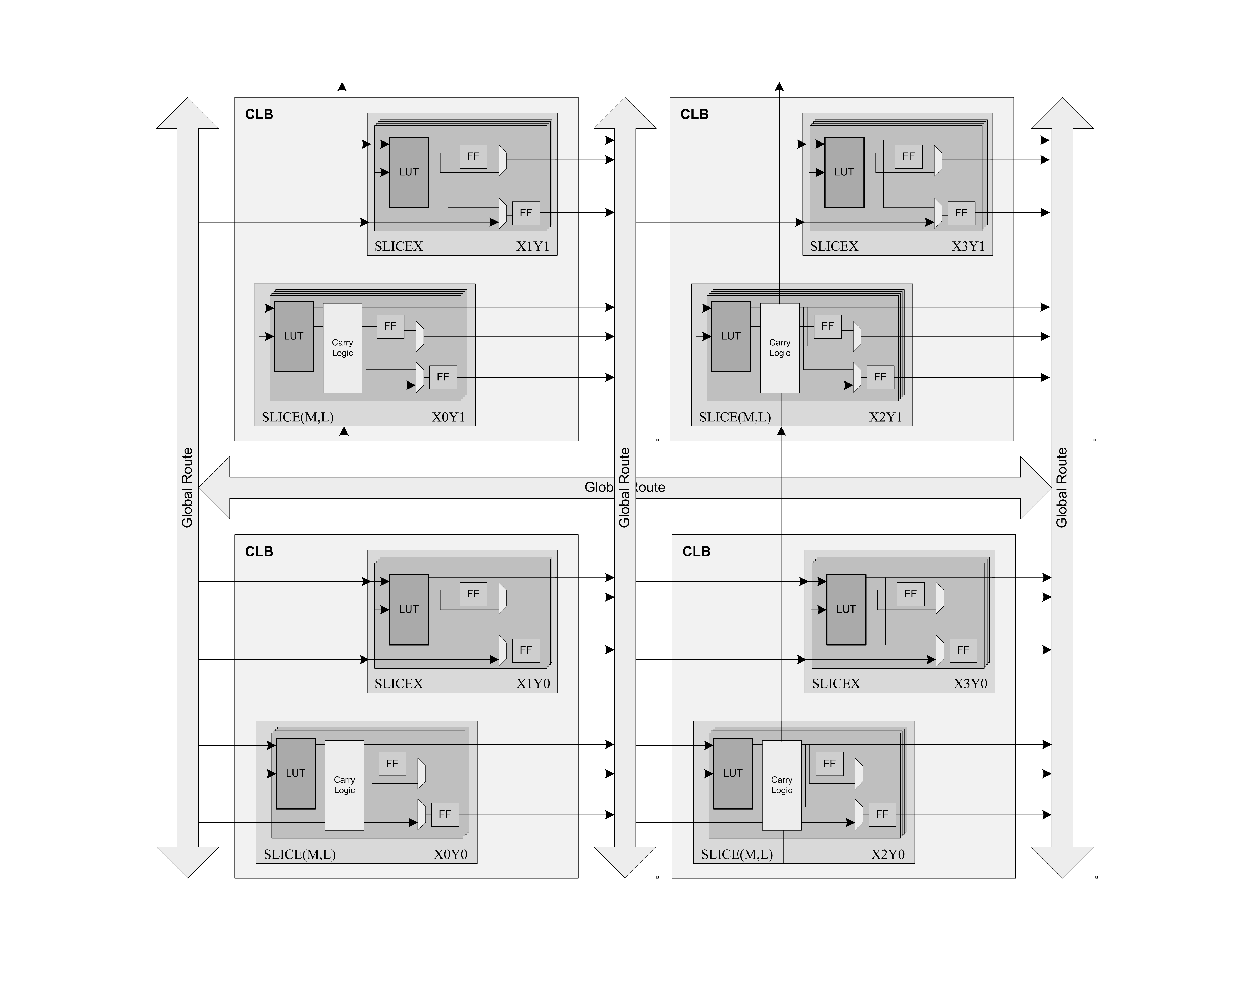
\includegraphics[scale=0.6]{img/spartan_arch}
\par\end{centering}
\caption{Bloque L\'{o}gico Configurable.}
\end{figure}

\end{doublespace}

Cada SLICE contiene cuatro LUTs, cuatro elementos de almacenamiento
(flip flop), un amplio n\'{u}mero de multiplexores y un bloque de
acarreo l\'{o}gico. Esos elementos son usados por todos los SLICEs
para proveer las funciones l\'{o}gicas, aritm\'{e}ticas y algunos
tipos de memoria ROM. Adicionalmente, algunos SLICEs pueden implementar
dos funciones adicionales: almacenar datos al adoptar la funci\'{o}n
de RAM distribuida y desplazar datos adoptando la funci\'{o}n de registro
de desplazamiento de 32 bits. Son llamados SLICEM (por Memoria), los
comunes son llamados SLICEL (Por L\'{o}gico).

La Figura describe con detalle la arquitectura de cada SLICE en un
CLB. Los multiplexores antes mencionados sirven para proveer la conectividad
entre los recursos l\'{o}gicos que rodean a los CLBs, mientras que
la red de elementos de acarreo en cadena dentro de los CLBs, hacen
la funci\'{o}n de ruteo para generar sumadores l\'{o}gicos m\'{a}s
eficientes.

\begin{doublespace}
\begin{figure}[H]
\begin{centering}
\includegraphics[scale=0.9]{img/slice_struct}
\par\end{centering}
\caption{Estructura detallada de un SLICE \cite{clb_ov}.}

\end{figure}

\end{doublespace}

Los dispositivos Spartan-6 cuentan con un gran n\'{u}mero de memorias
BRAM de 18Kb, las cuales est\'{a}n construidas por dos memorias controladas
independientemente de 9Kb cada una. Estas memorias son colocadas en
columnas, el n\'{u}mero total de ellas depende del tama\~{n}o del
dispositivo Spartan-6. Las memorias BRAM se pueden utilizar en cascada
para habilitar implementaciones de mayor tama\~{n}o de Kilo bits,
con un peque\~{n}o impacto en el timing. La Figura 6 muestra una BRAM
en cascada con dos distintos puertos de lectura y escritura.

\begin{figure}[H]
\begin{centering}
\includegraphics[scale=0.7]{img/bram_block}
\par\end{centering}
\caption{Block RAM de doble puerto \cite{clb_ov}.}

\end{figure}


\section{MATLAB como herramienta de dise\~{n}o de Alto Nivel.}

\subsection{Introducci\'{o}n a MATLAB.}

El nombre de esta herramienta proviene de recortar y unir las palabras
\textbf{MAT}rix \textbf{LAB}oratory (Laboratorio de Matrices), lo
cual nos da una referencia de la metodolog\'{\i}a que utiliza. MATLAB
es un sistema interactivo cuyo elemento b\'{a}sico son matrices las
cuales, no requieren ser dimensionadas. Est\'{a} enfocado a resolver
problemas t\'{e}cnicos computacionales a trav\'{e}s de un ambiente
completo donde los problemas y soluciones son expresados en una notaci\'{o}n
matem\'{a}tica familiar\cite{Matlab_overview}. Adem\'{a}s, la integraci\'{o}n
de herramientas para la adquisici\'{o}n de datos externos tales como
sonidos e im\'{a}genes, as\'{\i} como el an\'{a}lisis a trav\'{e}s
de aplicaciones de visualizaci\'{o}n como gr\'{a}ficas, hacen de este
lenguaje uno de los mas atractivos en el \'{a}rea de las ciencias
aplicadas.

Lo que hace de MATLAB una herramienta muy popular en el \'{a}mbito
acad\'{e}mico e industrial, es la rapidez con la que se pueden implementar
y resolver algoritmos de mediana a gran complejidad. Esto se debe
en gran medida a la facilidad que brinda el int\'{e}rprete interactivo
para crear scripts conocidos como Archivos-M (M-files, por sus siglas
en Ingl\'{e}s) que ayudan a describir sistemas con eficacia, as\'{\i}
como el gran n\'{u}mero de funciones predise\~{n}adas incluidas en
los complementos conocidos como <<cajas de herramienta>> o Toolboxes,
los cuales contienen colecciones de funciones para un gran rango de
disciplinas tales como procesamiento de se\~{n}ales, sistemas de control,
redes neuronales, l\'{o}gica difusa, por mencionar algunas. Todo esto
ayuda a que el usuario implemente sus modelos matem\'{a}ticos en cuesti\'{o}n
de horas y no d\'{\i}as, comparado con lenguajes compilados no interactivos
como C o Fortran.

\begin{figure}[H]
\begin{centering}
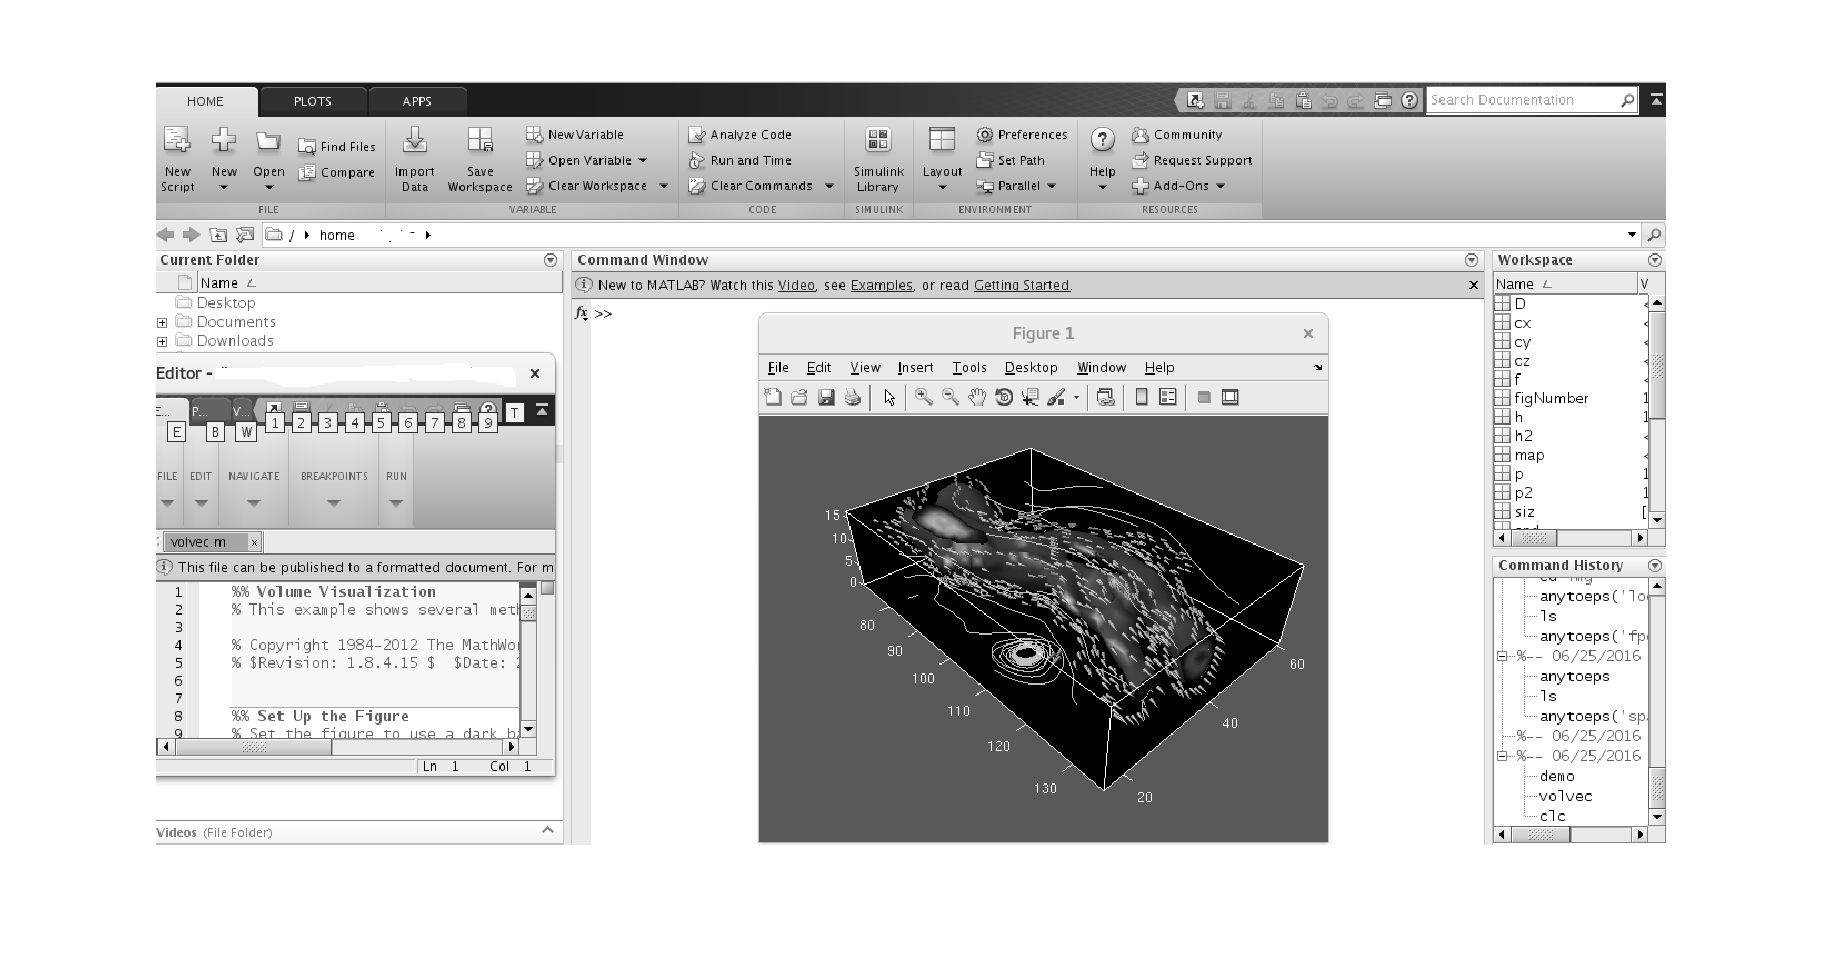
\includegraphics[scale=0.45]{img/matlab_env}
\par\end{centering}
\caption{Interfaz Gr\'{a}fica del Usuario de MATLAB.}

\end{figure}

MATLAB es considerado un lenguaje de programaci\'{o}n de alto nivel,
debido a la gran abstracci\'{o}n de datos con los que trabaja. Algunas
propiedades importantes de esta herramienta son:
\begin{itemize}
\item El tipo de datos por defecto es una matriz de doble precisi\'{o}n,
lo que significa que se pueden representar n\'{u}meros desde 0 a $1.7977e+308$.
\item Es un lenguaje orientado a objetos, lo cual resulta en una mejora
en el manejo de la complejidad de aplicaciones y estructuras de datos. 
\item Los algoritmos dise\~{n}ados en este paquete de software, pueden ser
convertidos a c\'{o}digo en lenguaje C, HDL y/o PLC, para ser ejecutados
en dispositivos embebidos.
\end{itemize}

\section{Flujo de dise\~{n}o DSP en FPGA.}

\newpage{}



\part{Marco metodol\'{o}gico.}

\section{Ejemplo 1: Procesamiento de Audio en tiempo real.}

\section{Ejemplo 2: Procesamiento de imagenes usando el kit Atlys como coprocesador.}

\newpage{}



\part*{Ap\'{e}ndice A: Conversi\'{o}n Anal\'{o}gico-Digital.}

\newpage{}

\part*{Ap\'{e}ndice B: Conversi\'{o}n Digital-Anal\'{o}gico.}

Para convertir una se\~{n}al digital a una anal\'{o}gica despu\'{e}s
de que se ha procesado por el sistema DSP, se utiliza un conversor
D/A (o DAC, por sus siglas en ingl\'{e}s). La manera en que este proceso
se lleva a cabo es interpolando los datos de las se\~{n}ales entre
las muestras tomadas, es decir, aplicando una aproximaci\'{o}n sucesiva
al valor de dichas muestras.

La manera m\'{a}s sencilla de convertir una se\~{n}al de anal\'{o}gico
a digital, es tomando las muestras de dicha se\~{n}al desde la memoria
donde el DSP las almacena, y transformarlas en un tren de impulsos,
como se muestra en la \textbf{Figura \ref{fig:Informaci=0000F3n-digital-convertida-1}}.\textbf{
}Despu\'{e}s, este mismo tren de pulsos, se hacer pasar por un filtro
pasa bajas, con la frecuencia de corte igual a la mitad de la frecuencia
de muestreo, cumpliendo el \emph{Teorema de Nyquist}.

\begin{figure}[H]
\begin{centering}
\includegraphics[scale=0.8]{img/impulse_train}
\par\end{centering}
\caption{Informaci\'{o}n digital convertida en un tren de impulsos \label{fig:Informaci=0000F3n-digital-convertida-1}.\cite{New1}}
\end{figure}

En otras palabras, la se\~{n}al original y el tren de impulsos tendr\'{a}n
espectros de frecuencia id\'{e}nticos, lo cual cumple con la \emph{frecuencia
de Nyquist} anteriormente descrita. En frecuencias m\'{a}s altas,
el tren de impulsos contiene una duplicaci\'{o}n de la se\~{n}al,
mientras que la se\~{n}al anal\'{o}gica original no contiene ninguna
informaci\'{o}n, suponiendo que el \emph{aliasing}\footnote{M\'{u}ltiples se\~{n}ales en tiempo continuo pueden producir series
de muestras id\'{e}nticas. A este fen\'{o}meno se le conoce como \emph{Aliasing}.
Cuando esto ocurre, el DAC no es cap\'{a}z de regenerar la se\~{n}al
de salida a menos que haya un filtro \emph{anti-aliasing }de por medio,
muestreando a una frecuencia mayor a la actual\cite{EECS_247}.}\textbf{\emph{ }}no ocurri\'{o}.

Mientras que este m\'{e}todo es matem\'{a}ticamente correcto, es dificil
generar esos trenes de pulsos tan estrechos entre si, utilizando componentes
electr\'{o}nicos. Para poder manejar esta dificultad, la mayor\'{\i}a
de los ADC operan manteniendo el \'{u}ltimo valor de entrada hasta
que se recibe otra muestra proveniente del DSP. A esto se le conoce
como \emph{retenci\'{o}n de \'{o}rden cero}, el equivalente del proceso
de \emph{muestra y retenci\'{o}n}\textbf{ }del DAC. La \emph{retenci\'{o}n
de orden cero }produce una se\~{n}al con apariencia de de escalera,
como se muestra en la \textbf{Figura} \ref{fig:Representaci=0000F3n-gr=0000E1fica-de-1}\footnote{Informaci\'{o}n sacada de \cite{chapter_3}.}. 

\begin{figure}[H]
\centering{}\includegraphics[scale=0.6]{img/staircase}\caption{Representaci\'{o}n gr\'{a}fica de una se\~{n}al producida por el efecto
de \emph{retenci\'{o}n de orden cero}\textbf{\emph{ }}en el proceso
de transformaci\'{o}n A/D \cite{chapter_3}\label{fig:Representaci=0000F3n-gr=0000E1fica-de-1}.}
\end{figure}

Hay diferentes formas de implementar estas conversiones D/A utilizando
componentes electr\'{o}nicos discretos y circuitos integrados, por
ejemplo\footnote{Para obtener m\'{a}s informaci\'{o}n sobre este tema, se puede referir
a \cite{binary_dacs_analogdev}, de donde se extrajo informaci\'{o}n
de esta secci\'{o}n.}
\begin{itemize}
\item \textbf{Ponderaci\'{o}n binaria: }Este DAC basado en resistores en
modo voltaje es usualmente la implementaci\'{o}n m\'{a}s simple utilizada
como referencia en los libros de texto (v\'{e}ase \textbf{Figura \ref{fig:Estructura-de-un-1}}).
No es inherentemente monol\'{\i}tico y es muy dificil de fabricar
de forma efic\'{a}z en grandes masas. Adem\'{a}s, la salida del DAC
utilizando el m\'{e}todo de ponderaci\'{o}n de voltaje binaria, cambia
con el c\'{o}digo de entrada. 
\begin{figure}[H]
\begin{centering}
\includegraphics[scale=0.4]{img/binary_res}
\par\end{centering}
\caption{\label{fig:Estructura-de-un-1}Estructura de un DAC resistivo de ponderaci\'{o}n
binaria. Imagen adaptada de: \cite{ad_resistive_one}}
\end{figure}
\item \textbf{Ponderaci\'{o}n binaria capacitiva en aproximaci\'{o}n sucesiva:
}El uso de una redistribuci\'{o}n de carga capacitiva ofrece la ventaja
de comportarse como un circuito de muestreo y retenci\'{o}n (SHA,
por sus siglas en ingl\'{e}s), por lo cual, ning\'{u}n circuito SHA
externo o incluso, alguna construcci\'{o}n monol\'{\i}tica SHA dentro
del circuito integrado, es requerido al utilizar esta estructura (v\'{e}ase
\textbf{Figura} \ref{fig:capacitivo_ponderacion_binaria-1}). 
\begin{figure}[H]
\begin{centering}
\includegraphics[scale=0.4]{img/capacitive_dac}
\par\end{centering}
\caption{\label{fig:capacitivo_ponderacion_binaria-1}Estructura de un DAC
capacitivo de ponderaci\'{o}n binaria.}
\end{figure}
\item \textbf{R-2R: }Una de las estructuras m\'{a}s comunes de DACs es la
muy conocida escalera R-2R, la cual consiste en una red de resistores
de s\'{o}lo dos diferentes valores, en una proporci\'{o}n de 2:1.
Un DAC de N bits requiere 2N resistores. El voltaje de salida se mantiene
siempre con la misma impedancia, (v\'{e}ase \textbf{Figura \ref{fig:DAC-R-2R-red-1}}).
\begin{figure}[H]
\begin{centering}
\includegraphics[scale=0.5]{img/r2r}
\par\end{centering}
\caption{\label{fig:DAC-R-2R-red-1}DAC R-2R red en escalera.}
\end{figure}
\end{itemize}
El voltaje salida de un DAC ideal se muestra en la \textbf{Figura
\ref{fig:Modelo-en-NGSpice-1}. }Para observar el c\'{o}digo Spice,
refierase al \textbf{Ap\'{e}ndice B \cite{spice_model}.}

\begin{figure}[H]
\begin{centering}
\includegraphics[scale=0.4]{img/ideal_dac}
\par\end{centering}
\caption{\label{fig:Modelo-en-NGSpice-1}Modelo en NGSpice de un DAC ideal
de 4 bits.}
\end{figure}

\newpage{}

\part*{Ap\'{e}ndice C: C\'{o}digo en Spice del DAC con respuesta ideal de
4 bits.}

\lstinputlisting[basewidth={0.5em},basicstyle={\ttfamily\small},breaklines=true,columns=flexible,keepspaces=true,language=Simula,morekeywords={WITH},tabsize=4]{src/ideal_dac.txt}

\newpage{}

\part*{Ap\'{e}ndice D: Script en Matlab de la Convoluci\'{o}n de dos vectores
de forma interactiva.}

\lstinputlisting[basewidth={0.5em},basicstyle={\ttfamily\small},breaklines=true,columns=flexible,keepspaces=true,language=Matlab,morekeywords={WITH},tabsize=4]{src/convolve_example.m}


\newpage{}

\bibliographystyle{unsrtnat}
\bibliography{bib/mainbib}

\end{document}
